\section{Overview}

Once the presented algorithms were implemented and packaged in DeepOF, there came the time to apply them to a real-world dataset. The model of choice, as introduced in chapter \ref{chap:introduction}, was Chronic Social Defeat Stress (CSDS), a widely adopted animal model on chronic stress and depression research. This acted as a positive control, where we had a clear idea of the expected shifts to detect, which would serve as validation for the provided package. Moreover, as significant symptoms of MDD are the deterioration of social functionality and a decline in social motivation, it also served as a good platform to test the detection of social interaction alterations in several ways.

Along these lines, the current chapter includes our paper titled \emph{Automatically annotated motion tracking identifies a distinct social behavioral profile following chronic social defeat stress}, published in \emph{Nature Communications} \cite{Bordes2023AutomaticallyStress}. In short, we here show how DeepOF can identify distinct stress-induced social and individual behavioral patterns, relying on both the annotation of pre-defined traits, and on unsupervised segmentation using the models presented in chapter \ref{chap:methods} \footnote{As introduced already in previous chapters, DeepOF offers three different encoder-decoder architectures (recurrent, TCN, transformers) and three time series segmentation approaches (VaDE, VQVAE, Contrastive+HMM). All results presented in this paper, however, relied on VaDE models with graph-like inputs and recurrent encoders/decoders. Results using other models did not substantially modify what was obtained, except for graph-input VQVAEs, which often diverged during training.}. Moreover, analyzing how global embedding shifts evolve over time reveals how these patterns are particularly noticeable at the onset of a novel social interaction, though they tend to diminish over time due to habituation in social settings.

We apply DeepOF to a variety of experimental settings, including single-animal open fields, social interaction (for which we use both single and multi-animal embeddings), and social avoidance tasks, and compare and interpret how the detected patterns vary across settings. Furthermore, while traditional social avoidance tasks (a set of univariate measures introduced in chapter~\ref{chap:introduction}) can detect stress-induced social behavioral differences, both supervised and unsupervised DeepOF pipelines offer a more comprehensive and detailed profile, which in addition requires lower experimental effort. Last but not least, a comprehensive statistical and visual interpretation of retrieved clusters is included.

\section{Contribution to the work}

I was the sole contributor of the DeepOF package, whose implementation was presented in the previous chapter and application is presented here. Moreover, I had the leading role in analyzing all the data presented in this chapter. Main figures 1 (except for mice drawings), 6, 7, as well as supplemental figures 1, 2, and 5--17 were conceived, designed, and coded by me. I did not take part in any of the animal experiments involved. I also wrote the full text in the manuscript (together with co-lead Joeri Bordes). First author order in the authors' list was randomized.

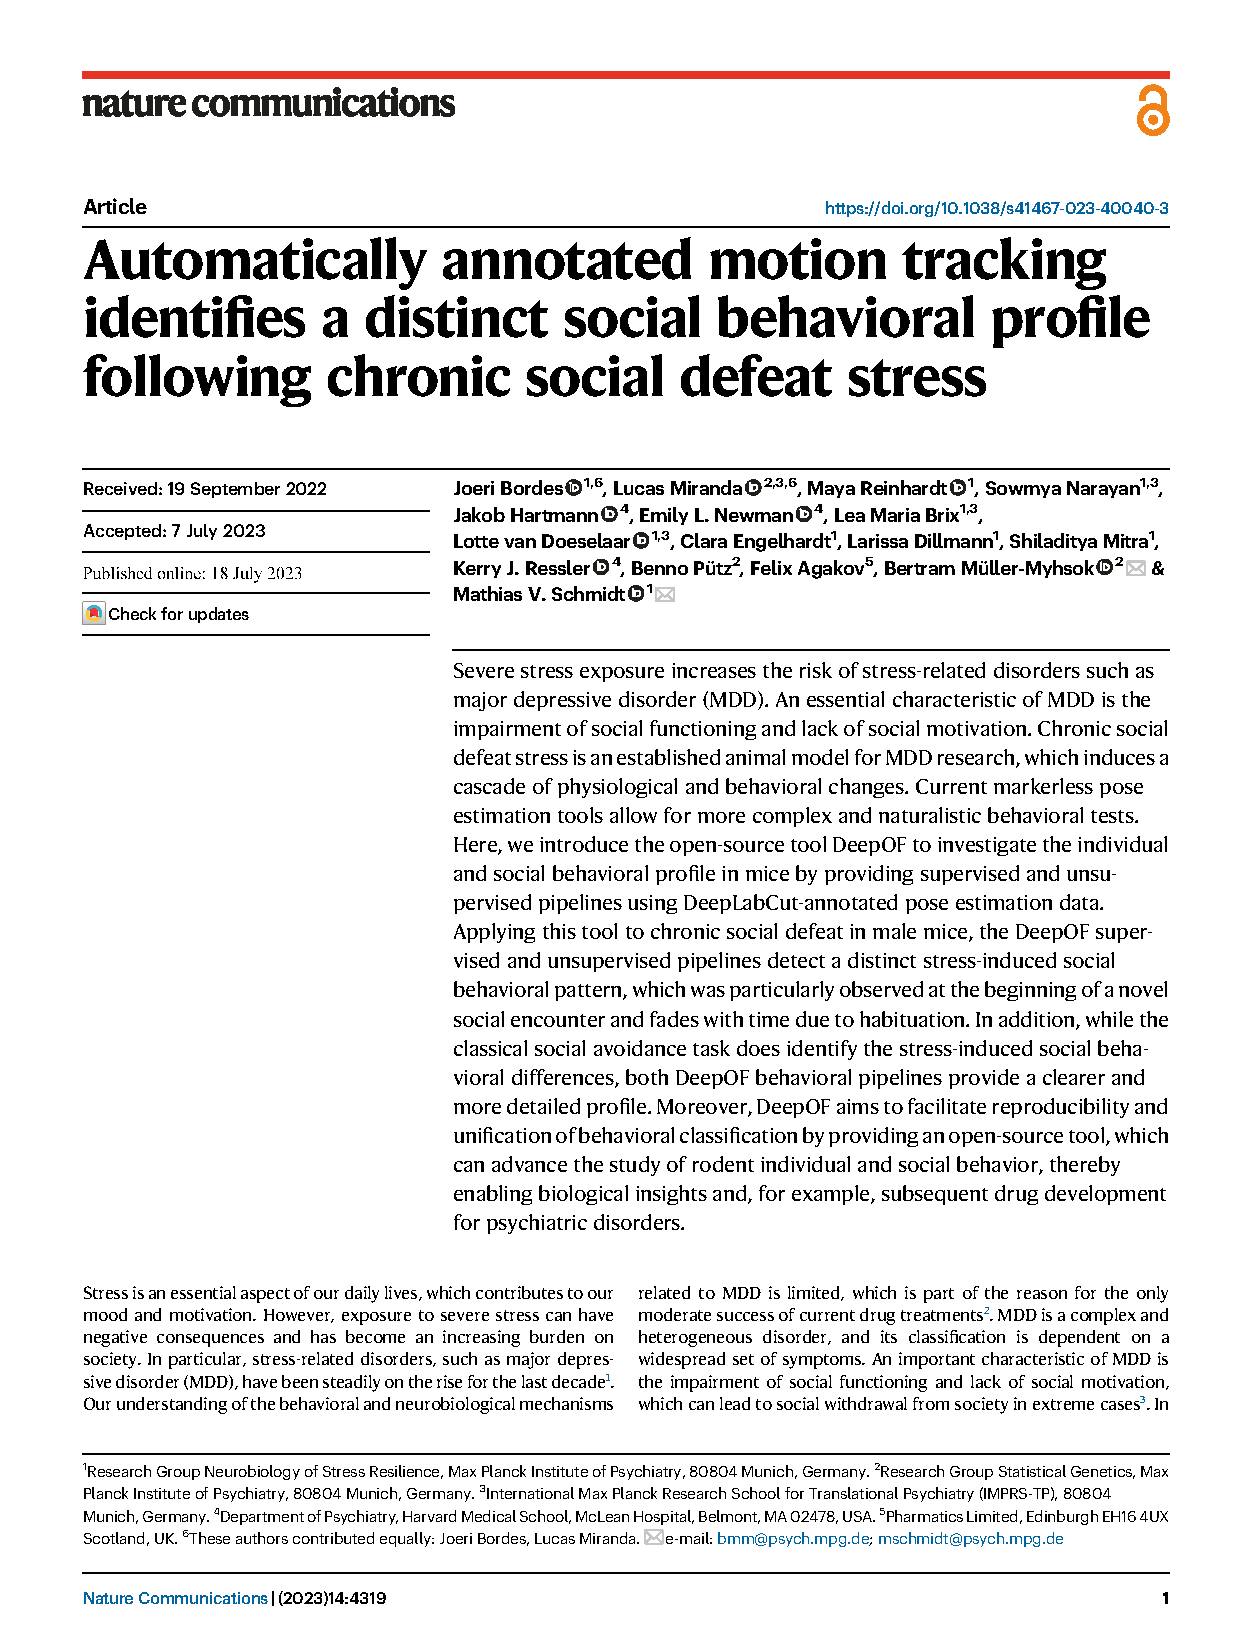
\includepdf[pages={-},
           addtolist={
           3, figure, \textbf{DeepOF workflow in detail:} an overview of data preprocessing and annotation pipelines, natcomm:fig1,
           4, figure, \textbf{Classical hallmarks for chronic social defeat stress}, natcomm:fig2,
           5, figure, \textbf{Social interaction binning yields more separable PCA projections than the social avoidance task}, natcomm:fig3,
           6, figure, \textbf{Top contributing behaviors in the social interaction task for 10 min total duration and time bins}, natcomm:fig4,
           7, figure, \textbf{Z-score correlation analysis and the exploration of susceptibility and resiliency}, natcomm:fig5,
           9, figure, \textbf{Single-animal unsupervised analyses identify different behavioral patterns between stressed and non-stressed mice during the SI task}, natcomm:fig6,
           10, figure, \textbf{SHAP analysis of unsupervised cluster assignments in the single-animal social interaction task}, natcomm:fig7
           },
           ]{Papers/natcomm.pdf}
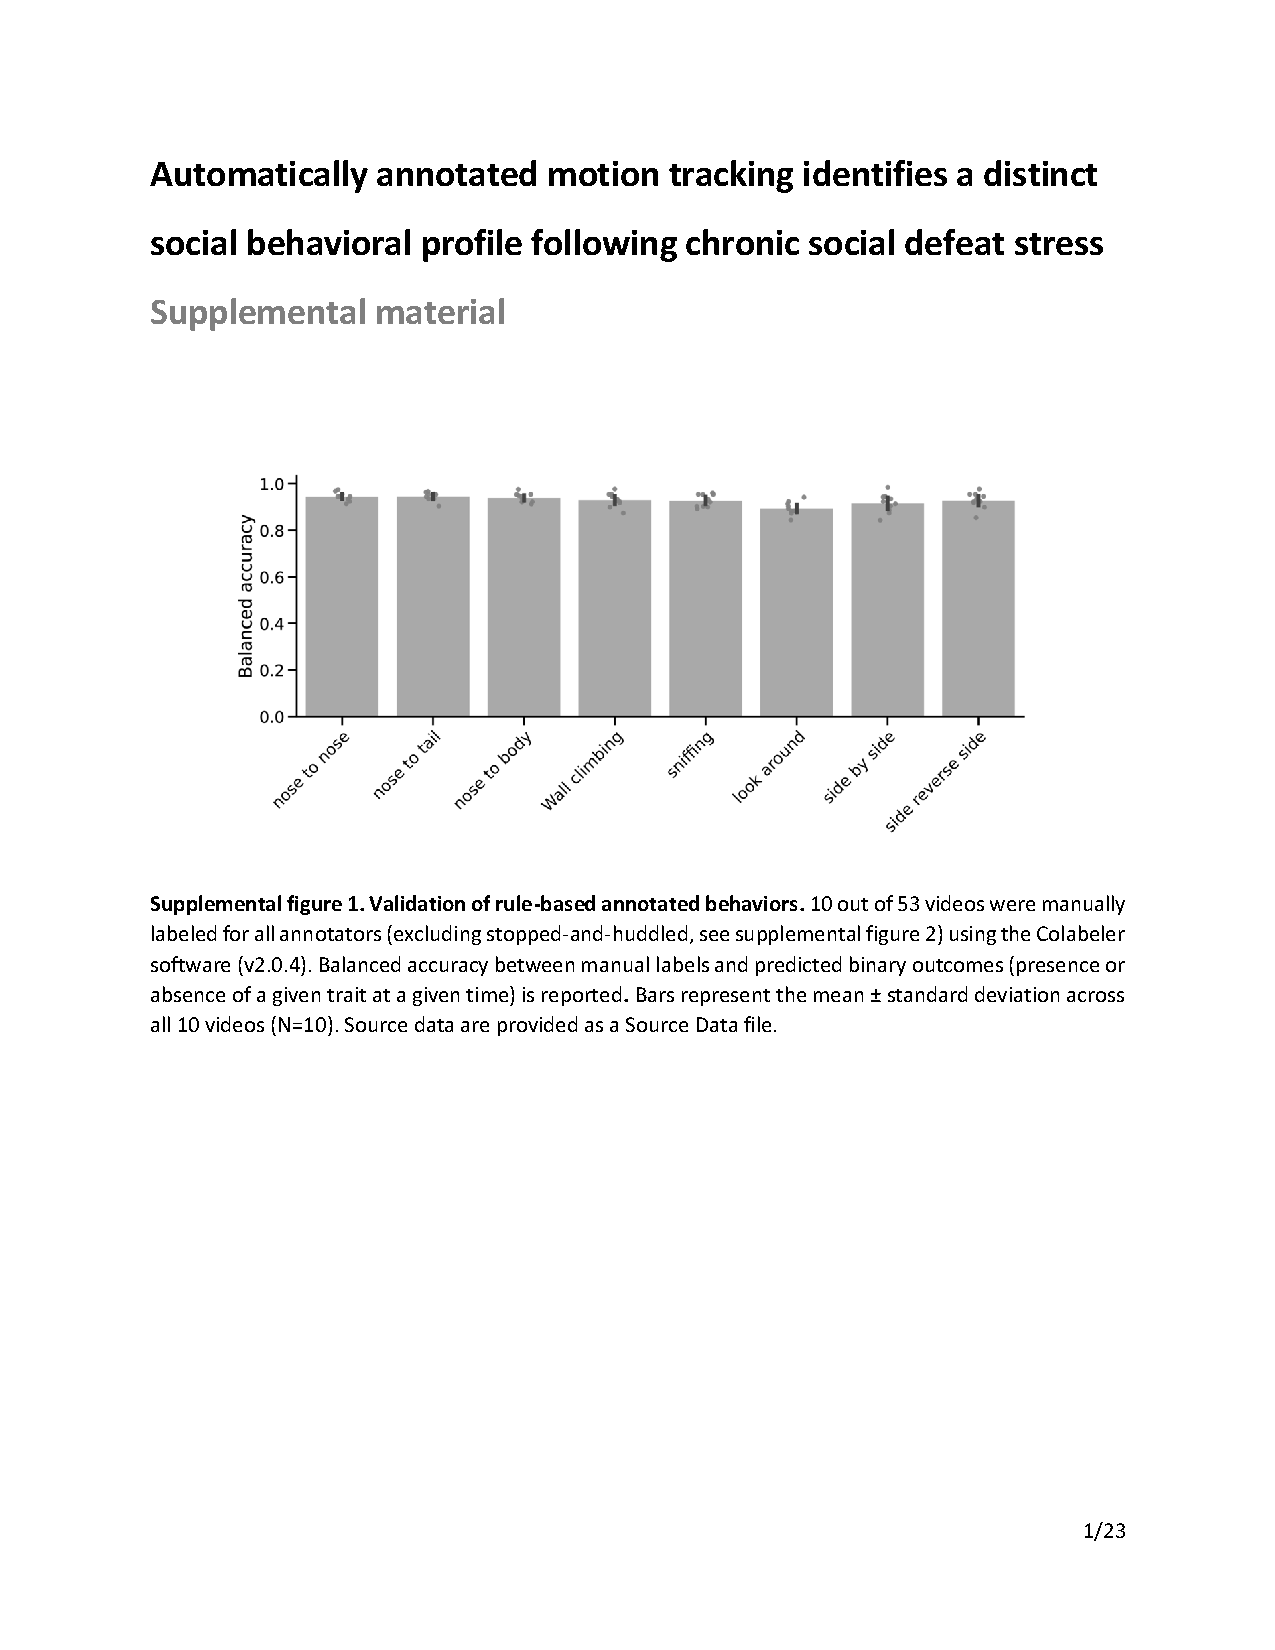
\includepdf[pages={-},
           addtolist={
           1, figure, \textbf{Validation of rule-based annotated behaviors in DeepOF}, natcomm:supfig1,
           2, figure, \textbf{Validation of the ``stopped and huddled" classifier provided within DeepOF}, natcomm:supfig2,
           3, table, \textbf{Default thresholds used by the annotation pipeline in DeepOF}, natcomm:suptab1,
           3, table, \textbf{Datasets used in the CSDS characterization study}, natcomm:suptab2,
           4, figure, \textbf{DeepOF behavioral classifiers in the open field task}, natcomm:supfig3,
           6, figure, \textbf{DeepOF other behavioral classifiers in the social interaction task for 10 min duration}, natcomm:supfig4,
           7, figure, \textbf{Multi-animal unsupervised analyses identify different two-mice behavioral patterns between arenas containing stressed and non-stressed mice during the SI task}, natcomm:supfig5,
           9, figure, \textbf{Single-animal unsupervised analyses identify different behavioral patterns between stressed and non-stressed mice during the OF task}, natcomm:supfig6,
           11, figure, \textbf{Single-animal unsupervised analyses identify mild behavioral differences between stressed and non-stressed mice during the SA task}, natcomm:supfig7,
           12, figure, \textbf{Global single-animal embeddings across non-overlapping time bins in the SI dataset}, natcomm:supfig8,
           13, figure, \textbf{Global multi-animal embeddings across non-overlapping time bins in the SI dataset}, natcomm:supfig9,
           14, figure, \textbf{Cluster enrichment per experimental condition in the second to fourth optimal bins for the single-animal embeddings on the SI task}, natcomm:supfig10,
           15, figure, \textbf{Cluster enrichment per experimental condition in the second to fourth optimal bins reported for the multi-animal embeddings on the SI task}, natcomm:supfig11,
           16, figure, \textbf{Spatial distribution of clusters obtained using single-animal embeddings in the SI task}, natcomm:supfig12,
           17, figure, \textbf{Spatial distribution of clusters obtained using multi-animal embeddings in the SI task}, natcomm:supfig13,
           18, figure, \textbf{Spatial distribution of clusters obtained in the OF task}, natcomm:supfig14,
           19, figure, \textbf{Correlation between behavioral entropy and stress physiology Z-score}, natcomm:supfig15,
           20, figure, \textbf{SHAP analysis of unsupervised cluster assignments in the multi-animal social interaction task}, natcomm:supfig16,
           22, figure, \textbf{SHAP analysis of unsupervised cluster assignments in the open field task}, natcomm:supfig17
           },
           ]{Papers/natcomm_supplemental.pdf}